\section{Background and Data}
\label{sec:background-data}
\label{sec:institutional-background}

Brazil is a useful setting for studying biometric voter registration because elections combine centralized administration, compulsory voting for most adults, and long-running investments in election technology. The \textit{Tribunal Superior Eleitoral} (\TSE{}) and the state-level \textit{Tribunais Regionais Eleitorais} (TREs) maintain the voter registry, organize elections, and supervise polling-day procedures. Voting itself is electronic and has been nationwide since 2000, a reform that substantially reduced residual votes and expanded de facto enfranchisement among poorer and less educated citizens, even as it also generated some new forms of voter error \citep{Fujiwara2015VotingTechnoloPolitica, Zucco2016TradingOldErrors}. In that institutional environment, biometric registration is best understood not as an isolated administrative tweak, but as a later stage of electoral modernization that changes both how voters are authenticated and how the electoral state manages the registry.

\subsection{Voting Administration and Biometric Registration}

Before biometric identification, voters typically authenticated themselves at the polling place with a voter registration card and another identity document, after which poll workers checked the information and released the electronic ballot. Biometric registration changed that interface. Under the biometric revision process, the electoral courts collect a voter's photograph, signature, and fingerprints in advance, and those data can then be used to verify identity at the polling place \citep{tse_revisao_eleitoral}. The program started with three pilot municipalities in 2008, formalized in \TSE{} Resolution No.~22,713 of February 28, 2008 \citep{tse_resolucao22713_2008}, and expanded over subsequent election cycles. By the 2024 municipal elections, the \TSE{} reported that 129.2 million electors, or 82.87\% of the electorate, had biometric records on file \citep{tse_biometria2024}.

The reform matters substantively because its effects are ambiguous ex ante. On one hand, biometric registration may improve record quality, reduce impersonation risk, and increase confidence in electoral administration. On the other hand, it requires voters to interact with the bureaucracy before election day, which can create compliance costs, especially where access to registration offices or information is uneven. Those two possibilities motivate the paper's focus on both administrative outcomes, such as electorate size and composition, and attitudinal outcomes, such as trust in elections and support for democracy.

\begin{figure}[htbp]
    \caption{Electoral Identification Materials}
    \label{fig:context-materials}
    \centering
    \begin{subfigure}[b]{0.48\textwidth}
        \centering
        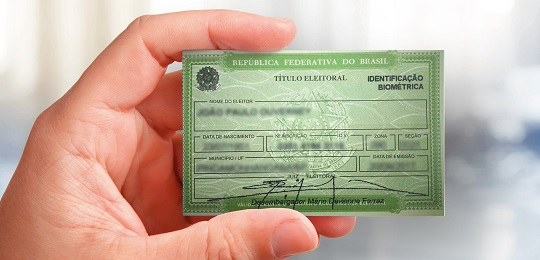
\includegraphics[width=\textwidth]{../resources/context/voter_id.jpeg}
        \caption{Voter identification card}
        \label{fig:voter-id}
    \end{subfigure}
    \hfill
    \begin{subfigure}[b]{0.48\textwidth}
        \centering
        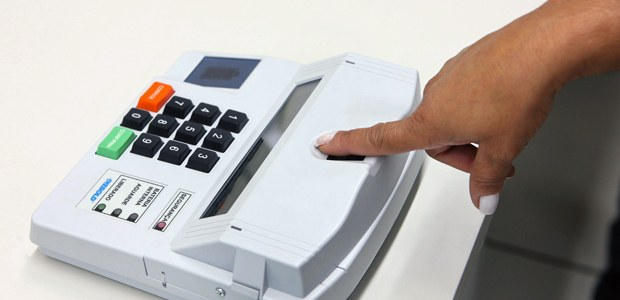
\includegraphics[width=\textwidth]{../resources/context/biometric_example.jpeg}
        \caption{Biometric verification at the polling place}
        \label{fig:biometric-verification}
    \end{subfigure}
\end{figure}

\subsection{Rollout and Treatment Coding}

The empirical design exploits the staggered municipal rollout of biometric registration. I define treatment timing as the first election year in which a municipality appears in the clean municipality-level biometric rollout file assembled from official \TSE{} resolutions, annexes, election-use attachments, and election-year electorate files. The clean first-treatment file contains 2,794 treated municipalities by 2018, while 2,777 municipalities remain untreated in the municipal panel through that year. Newly treated municipalities enter in waves: 3 in 2008, 57 in 2010, 239 in 2012, 465 in 2014, 779 in 2016, and 1,251 in 2018.

Figure~\ref{fig:bvr-rollout} summarizes those treatment waves directly. The visual makes clear that rollout was not only staggered, but increasingly concentrated in the later election cycles: adoption remains modest through 2012, then accelerates sharply in 2014, 2016, and especially 2018. By the end of the period, 2,794 municipalities in the clean panel, roughly half of all municipalities in the analysis sample, had entered the biometric regime. This timing structure is the core source of identifying variation in the paper. A companion spatial map appears in Appendix \hyperref[fig:appendix-bvr-treatment-map]{Figure~\ref*{fig:appendix-bvr-treatment-map}}, which shades municipalities by first observed BVR year, including hybrid implementation, and marks hybrid municipalities with diagonal hatching.

\begin{figure}[htbp]
    \caption{Municipal Rollout of Biometric Registration}
    \label{fig:bvr-rollout}
    \centering
    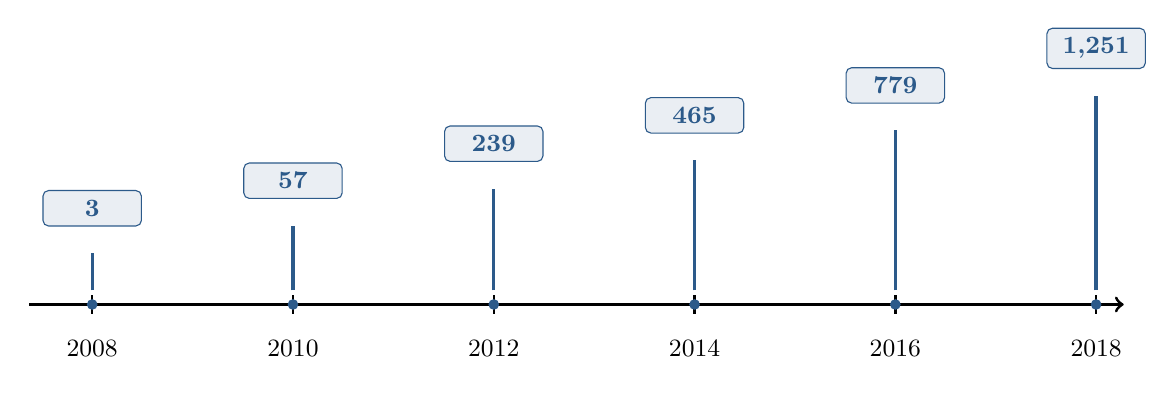
\begin{tikzpicture}[x=1cm,y=1cm]
\definecolor{BVRBlue}{HTML}{2C5A8A}
\draw[line width=1.1pt, ->] (0,0) -- (13.9,0);
\draw[line width=0.9pt] (0.80,0.12) -- (0.80,-0.12);
\filldraw[fill=BVRBlue, draw=BVRBlue] (0.80,0) circle (0.06);
\draw[BVRBlue, line width=1.2pt] (0.80,0.18) -- (0.80,0.65);
\node[anchor=south, draw=BVRBlue, fill=BVRBlue!10, rounded corners=2pt, minimum width=1.25cm, inner sep=3.5pt, text=BVRBlue, font=\bfseries\small] at (0.80,0.99) {3};
\node[anchor=north, font=\small] at (0.80,-0.33) {2008};
\draw[line width=0.9pt] (3.35,0.12) -- (3.35,-0.12);
\filldraw[fill=BVRBlue, draw=BVRBlue] (3.35,0) circle (0.06);
\draw[BVRBlue, line width=1.2pt] (3.35,0.18) -- (3.35,1.00);
\node[anchor=south, draw=BVRBlue, fill=BVRBlue!10, rounded corners=2pt, minimum width=1.25cm, inner sep=3.5pt, text=BVRBlue, font=\bfseries\small] at (3.35,1.34) {57};
\node[anchor=north, font=\small] at (3.35,-0.33) {2010};
\draw[line width=0.9pt] (5.90,0.12) -- (5.90,-0.12);
\filldraw[fill=BVRBlue, draw=BVRBlue] (5.90,0) circle (0.06);
\draw[BVRBlue, line width=1.2pt] (5.90,0.18) -- (5.90,1.47);
\node[anchor=south, draw=BVRBlue, fill=BVRBlue!10, rounded corners=2pt, minimum width=1.25cm, inner sep=3.5pt, text=BVRBlue, font=\bfseries\small] at (5.90,1.81) {239};
\node[anchor=north, font=\small] at (5.90,-0.33) {2012};
\draw[line width=0.9pt] (8.45,0.12) -- (8.45,-0.12);
\filldraw[fill=BVRBlue, draw=BVRBlue] (8.45,0) circle (0.06);
\draw[BVRBlue, line width=1.2pt] (8.45,0.18) -- (8.45,1.83);
\node[anchor=south, draw=BVRBlue, fill=BVRBlue!10, rounded corners=2pt, minimum width=1.25cm, inner sep=3.5pt, text=BVRBlue, font=\bfseries\small] at (8.45,2.17) {465};
\node[anchor=north, font=\small] at (8.45,-0.33) {2014};
\draw[line width=0.9pt] (11.00,0.12) -- (11.00,-0.12);
\filldraw[fill=BVRBlue, draw=BVRBlue] (11.00,0) circle (0.06);
\draw[BVRBlue, line width=1.2pt] (11.00,0.18) -- (11.00,2.21);
\node[anchor=south, draw=BVRBlue, fill=BVRBlue!10, rounded corners=2pt, minimum width=1.25cm, inner sep=3.5pt, text=BVRBlue, font=\bfseries\small] at (11.00,2.55) {779};
\node[anchor=north, font=\small] at (11.00,-0.33) {2016};
\draw[line width=0.9pt] (13.55,0.12) -- (13.55,-0.12);
\filldraw[fill=BVRBlue, draw=BVRBlue] (13.55,0) circle (0.06);
\draw[BVRBlue, line width=1.2pt] (13.55,0.18) -- (13.55,2.65);
\node[anchor=south, draw=BVRBlue, fill=BVRBlue!10, rounded corners=2pt, minimum width=1.25cm, inner sep=3.5pt, text=BVRBlue, font=\bfseries\small] at (13.55,2.99) {1,251};
\node[anchor=north, font=\small] at (13.55,-0.33) {2018};
\end{tikzpicture}

    \vspace{0.75em}
    \begin{minipage}{\textwidth}
        {\footnotesize \textbf{Note:} Each labeled count reports the number of municipalities whose first biometric election occurred in that election cycle. Counts are constructed from the project's clean municipality-level first-treatment file built from official \TSE{} rollout documents and electorate files. By 2018, 2,794 of the 5,571 municipalities in the clean panel had entered the biometric regime. \par}
    \end{minipage}
\end{figure}

One complication is partial or hybrid implementation. The project therefore separates the municipality-level first-treatment file from hybrid-status information. In the clean panel, 1,533 municipality-year observations in 2018 are flagged as hybrid, and those cases can be excluded or handled separately in robustness checks. This distinction matters because a municipality observed under a hybrid system is not equivalent to one that had fully transitioned to biometric verification earlier. The baseline treatment timing used in the municipal estimators is therefore conservative: it is anchored in the municipality-level first-treatment file rather than in a looser indicator of any biometric presence.

\subsection{Administrative Data}
\label{sec:data-and-measurement}

The main administrative dataset is a municipality-election panel built from official \TSE{} electorate files and the project's cleaned biometric-rollout file. The panel covers ten election years from 2000 through 2018 and contains 55,661 municipality-election observations across 5,571 municipalities in all 27 units of the federation \citep{tse_eleitorado}. At the municipality-election level, the core variables are the number of registered voters, its logarithm, the share of registered voters with lower schooling, the share with higher schooling, and parallel gender shares. Municipality identifiers are harmonized with the IBGE-TSE crosswalk stored in the repository, and the resulting panel is validated so that the final key is unique on `year_election + municipality_id` \citep{ibge_municipal}.

The electorate-composition measures come from \TSE{} tabulations by municipality, education, and gender. I classify ``low education'' as the set of categories below completed secondary schooling: illiterate, reads and writes, incomplete primary, and complete primary. ``High education'' includes incomplete secondary, complete secondary, incomplete higher education, and complete higher education. Importantly, the denominator for the reported shares is always the total municipality-level electorate, including cases with missing or unknown schooling. For that reason, the low- and high-education shares need not sum to one. This choice is deliberate: it prevents changes in missingness from being mechanically reallocated across the substantive education categories.

The administrative panel is designed to keep treatment coding and outcome construction transparent. Event time is defined relative to the first election year in which a municipality enters the biometric regime, while untreated municipalities remain in the sample as controls. Because the same cleaned panel also carries hybrid-status information, the administrative analysis can report a main specification and then assess whether results are sensitive to excluding municipality-years with documented hybrid implementation.

\subsection{Survey Data and Attitudinal Outcomes}

To study trust, democratic support, and beliefs about electoral integrity, the paper uses harmonized Brazil waves from the \LAPOP{} AmericasBarometer \citep{lapop_americasbarometer}. The core survey file currently available in the repository contains 10,009 respondents across six waves, 2008, 2010, 2012, 2014, 2017, and 2019, covering 25 states and 238 municipalities. The harmonized file preserves municipality and state names, interview timing, core demographics, and a consistent set of attitudinal variables. Those include trust in elections, trust in municipal government, broader institutional support, and several measures of democratic support and satisfaction.

The survey data complement the administrative panel in two ways. First, they allow the paper to ask whether biometric registration changed how citizens understand the integrity of elections and the legitimacy of democratic institutions, not just who remains on the voter rolls. Second, they make it possible to compare the timing of administrative change to shifts in attitudes measured after adoption. The municipal linkage is necessarily less comprehensive than in the \TSE{} panel, but it is still rich enough to support descriptive and difference-in-differences analyses that use the same treatment-timing logic while remaining explicit about survey coverage and precision limits.

Taken together, the administrative and survey data allow the paper to study biometric registration as both a registry reform and a political event. The administrative panel is well suited to measuring immediate changes in electorate size and composition around adoption, while the survey data allow the paper to examine whether those administrative changes coincide with greater confidence, skepticism, or backlash. Keeping those modules distinct at the data-construction stage is useful analytically: it makes clear which results come from population-wide administrative records and which come from sampled attitudes, and it helps keep causal claims proportional to the underlying evidence.
